\section{Introduction}

One of the major trends in city planning is the introduction of light rail transit networks. However, when spatial development has previously been based on the automobile, the often low densities of residences and activities may not provide ideal conditions for a transit line. To facilitate the integration of a new transit line into the existing road network, a common approach is to include park-and-ride facilities around transit stations, allowing car-based access to the transit line.

Sioux Falls, South Dakota, is a city that has experienced rapid growth in recent years. The city, which had a population of 125,000 at the start of the century, now has a population of over 200,000 within an area of 210 km$^2$\footnote{\url{https://en.wikipedia.org/wiki/Sioux_Falls,_South_Dakota}}. In terms of population, this is comparable to the city of Geneva, which has multiple light rail lines, suburban train lines, and a dense bus network (although Geneva covers only 16 km$^2$\footnote{\url{https://fr.wikipedia.org/wiki/Gen\%C3\%A8ve}}). In comparison, Sioux Falls' public transport relies only on 9 bus lines, which run just 6 days a week, and on-demand transport\footnote{\url{https://siouxareametro.info/bus}}. Additionally, Sioux Falls' road network inspired the homonymous benchmark network, which is well-known in traffic engineering for its small size and typical grid structure.

\begin{figure}
    \centering
    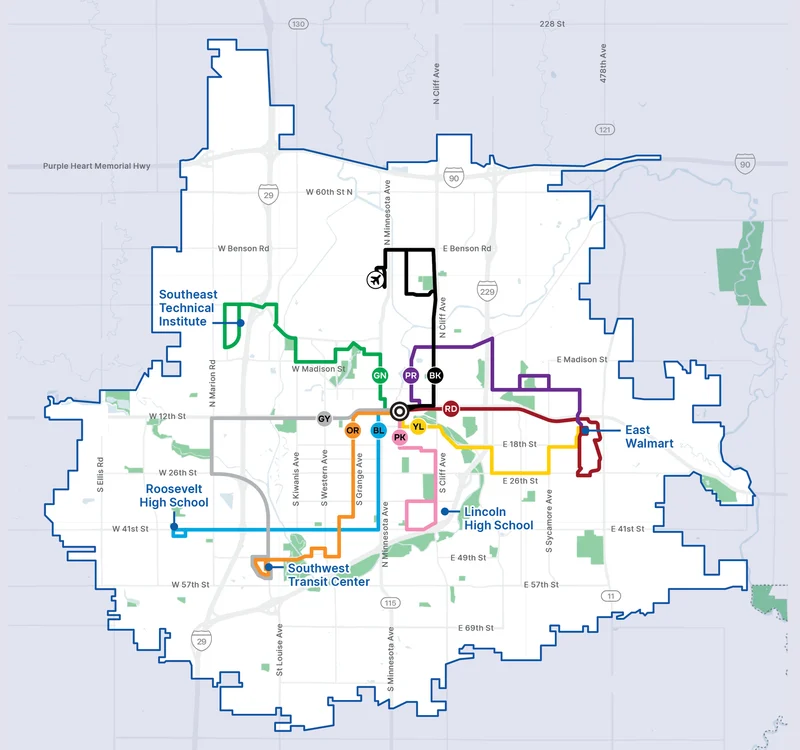
\includegraphics[keepaspectratio,width=0.45\textwidth]{Figures/siouxfalls_bus_network.png}
    \caption{Sioux Falls' current bus network.}
    \label{fig:sioux_falls_bus_network}
\end{figure}

In a hypothetical scenario, the city of Sioux Falls is considering the construction of a light rail line to improve public transportation usage. This study will analyze the potential decrease in traffic from converting one existing bus line into a light rail line, as well as the introduction of park-and-ride facilities at the stations. To do this, we will solve for traffic at \textit{User Equilibrium} (UE) in the benchmark network, and then simulate the introduction of the new light rail line as new links between the nodes, with the restriction that a user may use it only if both their origin and destination are along the line. Finally, the introduction of park-and-ride facilities will be simulated by replacing the previous constraint and allowing users to access the light rail line if either their origin or destination is along the line.

Future research could consider parking and ticket fares, the inconvenience of having to change modes, and the waiting time to be included as a generic cost added to the travel time on the transit line. The possibility of including park-and-ride facilities at only some stations, limiting the capacity of the parking lots, more detailed cost computations (e.g., precise calculations, inclusion of fuel cost in individual transport links), and a sensitivity analysis on the value of the generic cost would, if time allows, be interesting additions to the study.